\documentclass[11pt,a4paper]{article}

% ------------------------------------------------------------------ packages
\usepackage[T1]{fontenc}
\usepackage[utf8]{inputenc}
\usepackage{newtxtext,newtxmath}
\usepackage[margin=2.5cm]{geometry}
\usepackage{microtype}
\usepackage{amsmath,mathtools}
\usepackage{graphicx}
\usepackage{booktabs}
\usepackage{multirow}
\usepackage[table]{xcolor}
\usepackage{siunitx}
\usepackage{subcaption}
\usepackage{caption}
\usepackage{enumitem}
\usepackage{tikz}
\usetikzlibrary{arrows.meta,positioning,fit,backgrounds,calc}
\usepackage[numbers,sort&compress]{natbib}
\usepackage[colorlinks=true,linkcolor=accent,citecolor=accent,urlcolor=accent]{hyperref}
\usepackage[capitalise,noabbrev]{cleveref}

\definecolor{accent}{HTML}{256ABF}
\definecolor{sOne}{HTML}{2A78D6}
\definecolor{sTwo}{HTML}{EB6834}
\definecolor{sThree}{HTML}{1BAF7A}
\definecolor{inkTwo}{HTML}{52514E}
\definecolor{soft}{HTML}{F0EFEC}
\definecolor{softBlue}{HTML}{CDE2FB}

\captionsetup{font=small,labelfont=bf,labelsep=period}
\captionsetup[sub]{font=small}
\setlist{itemsep=2pt,topsep=4pt}
\sisetup{detect-all,group-separator={,},group-minimum-digits=4}
\graphicspath{{figures/}}
\renewcommand{\topfraction}{0.9}
\renewcommand{\textfraction}{0.1}
\renewcommand{\floatpagefraction}{0.8}

% numbers generated from reports/ by scripts/make_figures.py
% generated by scripts/make_figures.py, do not edit
\newcommand{\numAblEarlyStopped}{4}
\newcommand{\numAblHandsOnly}{+0.0}
\newcommand{\numAblNoAugment}{-1.3}
\newcommand{\numAblNoCanonical}{-3.8}
\newcommand{\numAblNoHandlocal}{-0.8}
\newcommand{\numAblNoLips}{+0.5}
\newcommand{\numAblNoVelocity}{-1.7}
\newcommand{\numAblPad}{+1.2}
\newcommand{\numAblTNineSix}{-0.8}
\newcommand{\numAblTThreeTwo}{+0.2}
\newcommand{\numAblXyz}{-1.1}
\newcommand{\numAslClasses}{250}
\newcommand{\numAslDurMedian}{0.73}
\newcommand{\numAslEnsFOne}{66.8}
\newcommand{\numAslEnsTop}{67.4}
\newcommand{\numAslFramesMedian}{22}
\newcommand{\numAslLgbmDrop}{11}
\newcommand{\numAslLgbmTest}{33.8}
\newcommand{\numAslLgbmVal}{45.2}
\newcommand{\numAslLogregChance}{105}
\newcommand{\numAslLogregDrop}{6}
\newcommand{\numAslLogregTest}{42.1}
\newcommand{\numAslLogregVal}{47.9}
\newcommand{\numAslNoHandPct}{34.1}
\newcommand{\numAslSamples}{94,477}
\newcommand{\numAslSigners}{21}
\newcommand{\numBrowserDiff}{2\times10^{-6}}
\newcommand{\numBrowserSame}{40/40}
\newcommand{\numExampleAcc}{70.0}
\newcommand{\numFpBrowser}{16}
\newcommand{\numFpNative}{7.8}
\newcommand{\numFpSizeMB}{8.3}
\newcommand{\numFtFive}{30.0}
\newcommand{\numFtTwentyFive}{50.6}
\newcommand{\numFullHandFrames}{16}
\newcommand{\numGainAll}{-2.0}
\newcommand{\numGainFew}{1.4}
\newcommand{\numGapTestClip}{68.3}
\newcommand{\numGapTestPartnerIn}{71.8}
\newcommand{\numGapTestPartnerInN}{17}
\newcommand{\numGapTestPartnerOut}{64.7}
\newcommand{\numGapTestPerSigner}{67.9}
\newcommand{\numGapTestPerSignerSem}{2.0}
\newcommand{\numGapTestReweighted}{70.2}
\newcommand{\numGapTestSigners}{40}
\newcommand{\numGapTopThreeShare}{75}
\newcommand{\numGapValClip}{77.2}
\newcommand{\numGapValPartnerInN}{6}
\newcommand{\numGapValPerSigner}{72.7}
\newcommand{\numGapValPerSignerSem}{2.5}
\newcommand{\numGapValSigners}{9}
\newcommand{\numGruBrowser}{8}
\newcommand{\numGruParams}{1.43}
\newcommand{\numGruSignerStd}{3.9}
\newcommand{\numGruTestTop}{63.0 $\pm$ 0.5}
\newcommand{\numGruTestTopFive}{84.0}
\newcommand{\numGruTestTopMean}{63.0}
\newcommand{\numGruValTopMean}{65.8}
\newcommand{\numHandlessOutside}{2.4}
\newcommand{\numHandlessSample}{5,000}
\newcommand{\numIntLatency}{33}
\newcommand{\numIntNative}{16.5}
\newcommand{\numIntShrink}{3.3}
\newcommand{\numIntSizeMB}{2.5}
\newcommand{\numIntSlowdown}{2.1}
\newcommand{\numJsParity}{$3\times10^{-6}$}
\newcommand{\numLcMin}{5}
\newcommand{\numLeakGap}{16.9}
\newcommand{\numLeakRandom}{81.7}
\newcommand{\numLeakSigner}{64.8}
\newcommand{\numLongVal}{67.5}
\newcommand{\numLowlrTwentyFive}{46.3}
\newcommand{\numLsfbAllGlosses}{4,657}
\newcommand{\numLsfbAllInstances}{120,739}
\newcommand{\numLsfbAllSigners}{99}
\newcommand{\numLsfbClasses}{100}
\newcommand{\numLsfbDroppedPct}{0.6}
\newcommand{\numLsfbDurMedian}{0.32}
\newcommand{\numLsfbEnsFOne}{66.8}
\newcommand{\numLsfbEnsTop}{70.9}
\newcommand{\numLsfbFps}{50}
\newcommand{\numLsfbFramesMedian}{16}
\newcommand{\numLsfbFreezeCiHi}{-1.2}
\newcommand{\numLsfbFreezeCiLo}{-2.3}
\newcommand{\numLsfbFreezeDiff}{-1.7}
\newcommand{\numLsfbFreezeP}{p<0.001}
\newcommand{\numLsfbFreezeTest}{66.6}
\newcommand{\numLsfbFreezeTestFOne}{62.0}
\newcommand{\numLsfbFreezeVal}{75.6}
\newcommand{\numLsfbFtCiHi}{-1.4}
\newcommand{\numLsfbFtCiLo}{-2.8}
\newcommand{\numLsfbFtDiff}{-2.1}
\newcommand{\numLsfbFtP}{p<0.001}
\newcommand{\numLsfbFtTest}{66.2}
\newcommand{\numLsfbFtTestFOne}{61.7}
\newcommand{\numLsfbFtVal}{74.9}
\newcommand{\numLsfbLogregTest}{49.0}
\newcommand{\numLsfbLogregTestFOne}{40.9}
\newcommand{\numLsfbLogregVal}{57.0}
\newcommand{\numLsfbMedianPerClass}{185}
\newcommand{\numLsfbNoHandPct}{1.5}
\newcommand{\numLsfbScratchTest}{68.3}
\newcommand{\numLsfbScratchTestFOne}{63.9}
\newcommand{\numLsfbScratchVal}{77.0}
\newcommand{\numLsfbTopTenShare}{32}
\newcommand{\numMissHighAcc}{52.0}
\newcommand{\numMissHighShare}{30}
\newcommand{\numMissLowAcc}{76.5}
\newcommand{\numNoseAsl}{0.40}
\newcommand{\numNoseLsfbCorr}{0.43}
\newcommand{\numNoseLsfbFourThree}{0.57}
\newcommand{\numNoseLsfbRaw}{0.76}
\newcommand{\numPartHandFrames}{24}
\newcommand{\numProbeAll}{38.3}
\newcommand{\numRefValTop}{68.3}
\newcommand{\numScratchFive}{27.4}
\newcommand{\numScratchLeadAll}{2.0}
\newcommand{\numScratchTwentyFive}{51.5}
\newcommand{\numShortAcc}{59}
\newcommand{\numSignerMax}{69.5}
\newcommand{\numSignerMin}{61.9}
\newcommand{\numTrGruCiHi}{2.9}
\newcommand{\numTrGruCiLo}{0.9}
\newcommand{\numTrGruClipCiHi}{2.2}
\newcommand{\numTrGruClipCiLo}{1.4}
\newcommand{\numTrGruDiff}{1.8}
\newcommand{\numTrGruMcnemar}{p<0.001}
\newcommand{\numTrParams}{2.16}
\newcommand{\numTrSignerStd}{3.3}
\newcommand{\numTrTestTop}{64.8 $\pm$ 0.4}
\newcommand{\numTrTestTopFive}{84.0}
\newcommand{\numTrTestTopMean}{64.8}
\newcommand{\numTrValTopMean}{68.2}
\newcommand{\numTypicalAcc}{77}
\newcommand{\numWorstClasses}{\textsc{there} (3\,\%), \textsc{finger} (12\,\%), \textsc{go} (18\,\%)}


\usepackage{xspace}
\newcommand{\ie}{i.e.\@\xspace}
\newcommand{\eg}{e.g.\@\xspace}

% ------------------------------------------------------------------ title
\title{\textbf{Pose-Based Isolated Sign Recognition in the Browser:\\
Signer-Independent Evaluation and Cross-Lingual Transfer\\ from ASL to French Belgian Sign Language}}
\author{Anais Azouaoui}
\date{}

\begin{document}
\maketitle

\begin{abstract}
Pose-based isolated sign recognition is commonly evaluated on random splits and rarely deployed on
consumer hardware. We study it under the condition that matters in practice: recognising signs
produced by people absent from the training data. A single preprocessing function, shared by
training and by a JavaScript port, converts MediaPipe Holistic landmarks into features for a
2.2\,M-parameter convolution--Transformer. On Google ISLR (\numAslClasses{} American Sign Language
signs, \numAslSigners{} signers), the model reaches \numTrTestTop{}\,\% top-1 accuracy on four
unseen signers, against \numGruTestTop{}\,\% for a bidirectional GRU and \numAslLogregTest{}\,\% for a statistical
baseline; a random split overestimates this accuracy by \numLeakGap{} points. One-factor ablations
identify the canonical dominant hand as the most influential preprocessing step. On LSFB-ISOL
(\numLsfbClasses{} glosses of French Belgian Sign Language), initialising the model from ASL brings
no gain at any training-set size, from \numLcMin{} examples per sign to the full corpus
and is slightly but significantly harmful with all data (\numLsfbFtTest{}\,\% against
\numLsfbScratchTest{}\,\% from scratch on 40 unseen signers). We also
document three silent failure modes of such pipelines: augmentations cancelled by normalisation,
anisotropic coordinates in anamorphic video, and feature outliers that break INT8 quantisation.
In the browser, the model classifies a sign in \numFpBrowser{}\,ms on one CPU thread and
reproduces the PyTorch predictions on every tested clip.

\end{abstract}

\section{Introduction}
\label{sec:intro}

Sign languages are natural languages with their own lexicon and grammar, used by millions of Deaf
and hard-of-hearing people. Automatic sign language processing covers tasks of increasing
difficulty: \emph{isolated} sign recognition (one sign per clip, closed vocabulary), continuous
recognition, and translation to and from spoken languages
\citep{bragg2019interdisciplinary,koller2020survey,yin2021including}. This report addresses
isolated recognition only. The distinction is not merely terminological: a classifier over a few
hundred glosses ignores the grammar of the language, its use of space and its non-manual markers,
and therefore cannot translate \citep{yin2021including}.

\emph{Pose-based} approaches first extract body, hand and face landmarks with an off-the-shelf
estimator such as MediaPipe Holistic
\citep{lugaresi2019mediapipe,bazarevsky2020blazepose,zhang2020mediapipehands,kartynnik2019facemesh},
then classify the resulting keypoint sequence. Compared with models operating on RGB video, they
are compact, largely insensitive to background and appearance, and allow inference without
transmitting video, which protects the privacy of users. The Google Isolated Sign Language
Recognition (ISLR) competition \citep{kaggle_islr} established this setting with
\numAslSamples{} landmark sequences of \numAslClasses{} American Sign Language (ASL) signs.

Three questions remain insufficiently addressed in this setting. They structure the report.
\begin{description}[leftmargin=1.2em,labelindent=0pt]
  \item[RQ1 Generalisation.] How accurately do pose-based models recognise signs produced by
        people absent from the training data, and how much does a random split overestimate this
        accuracy?
  \item[RQ2 Transfer.] Does pre-training on ASL, a comparatively well-resourced sign language,
        improve recognition in French Belgian Sign Language (LSFB), in particular when few
        labelled examples are available?
  \item[RQ3 Deployment.] Can the complete pipeline run in real time in a web browser on a laptop
        CPU while reproducing the predictions of the trained model?
\end{description}

\paragraph{Contributions.}
\begin{itemize}
  \item A single, unit-tested preprocessing function shared by training, evaluation and a
        JavaScript port, whose outputs match the reference implementation within \numJsParity{}
        (\cref{sec:method}).
  \item A signer-independent comparison of a statistical baseline, a bidirectional GRU and a
        convolution--Transformer on \numAslClasses{} ASL signs over three seeds, with paired
        significance tests, a measurement of split leakage and one-factor ablations
        (\cref{sec:results-asl,sec:ablations}).
  \item A controlled transfer study from ASL to LSFB, with learning curves from \numLcMin{}
        examples per sign to the full corpus and a linear probe of the pre-trained encoder
        (\cref{sec:transfer}).
  \item A fully client-side demo that classifies a sign in \numFpBrowser{}\,ms, and an analysis
        of INT8 quantisation, which first degrades accuracy because of feature outliers and,
        once corrected, remains slower on CPU (\cref{sec:efficiency}).
\end{itemize}

\Cref{sec:related} reviews related work. \Cref{sec:data,sec:method,sec:protocol} describe the
data, the method and the evaluation protocol. \Cref{sec:results} reports the results,
\cref{sec:discussion} discusses them together with their limitations, and
\cref{sec:conclusion} answers the three research questions.

\section{Related work}
\label{sec:related}

\paragraph{Isolated sign recognition datasets.}
Large ASL vocabularies are available in WLASL \citep{li2020wlasl} (2{,}000 glosses collected from
the web), MS-ASL \citep{joze2019msasl} and ASL Citizen \citep{desai2023aslcitizen}; the latter is
community-sourced, collected with explicit consent and provided with signer-independent splits.
BSL-1K \citep{albanie2020bsl1k} mines British Sign Language signs from broadcast footage using
mouthing cues. The Google ISLR competition \citep{kaggle_islr} released MediaPipe landmarks only,
recorded by 21 participants on smartphones, which removes the need to store video. For sign
languages related to French, LSFB-ISOL and LSFB-CONT \citep{fink2021lsfb} are derived from the LSFB
corpus \citep{meurant2015corpus}. On LSFB-ISOL, \citet{fink2023dictionary} train a two-layer
Transformer on MediaPipe landmarks of 700 glosses with more than 20 examples each, under a
signer-independent split, and report 54\,\% top-1 and 83\,\% top-10 accuracy. No subset of
LSFB-ISOL has become a standard benchmark, so our results on the 100 most frequent glosses cannot be
compared directly with theirs. MEDIAPI-SKEL \citep{bull2020mediapi} and
Dicta-Sign-LSF-v2 \citep{belissen2020dictasign} provide continuous French Sign Language (LSF) with
skeletons or annotations but no isolated-sign benchmark.

\paragraph{Pose-based models.}
Skeleton sequences have been classified with spatio-temporal graph convolutions
\citep{yan2018stgcn,jiang2021samslr,tunga2021gcnbert}, with Transformers operating directly on
keypoints \citep{bohacek2022spoter}, and with self-supervised pre-training of hand representations
\citep{hu2021signbert}. The strongest solutions of the Google ISLR competition combined depthwise
temporal convolutions with a few self-attention layers, a design close to the Conformer used in
speech recognition \citep{gulati2020conformer}, trained for several hundred epochs with strong
regularisation and averaged over ensembles of models. Our convolution--Transformer follows this
design at a smaller scale. Recurrent networks \citep{cho2014gru} remain a light and competitive baseline.

\paragraph{Transfer across sign languages.}
Sign languages share articulatory parameters (handshape, movement, location), which suggests that
features learned on a large corpus may transfer to a smaller one \citep{yosinski2014transferable}.
Large-scale pre-training improves recognition on smaller datasets of the \emph{same} language
\citep{albanie2020bsl1k}. Transfer between distinct sign languages from pose data alone has
received less attention; we provide a controlled study with learning curves.

\paragraph{Responsible deployment.}
Following \citet{bragg2019interdisciplinary} and \citet{yin2021including}, we describe the system as
isolated sign recognition, document its limitations in a model card \citep{mitchell2019modelcards}
and process video locally on the device of the user.

\section{Data}
\label{sec:data}

\begin{table}[t]
  \centering
  \caption{Datasets after conversion to the unified format. Durations are medians; ``no hand'' is
  the share of frames in which neither hand is detected.}
  \label{tab:datasets}
  \small
  \begin{tabular}{lrrrcrrrr}
\toprule
 & & & & Signers & Clips & & & No \\
Dataset & Classes & Clips & Signers & tr/val/test & per class & Duration & fps & hand \\
\midrule
ASL (Google ISLR) & 250 & 94,477 & 21 & 14/3/4 & 299--415 & 0.73\,s & 30 & 34\,\% \\
LSFB-ISOL & 100 & 55,286 & 99 & 50/9/40 & 216--3293 & 0.32\,s & 50 & 2\,\% \\
\bottomrule
\end{tabular}

\end{table}

\paragraph{Google ISLR (ASL).}
The competition data \citep{kaggle_islr} contain \numAslSamples{} sequences of \numAslClasses{} ASL
signs produced by \numAslSigners{} participants. Each frame provides the 543 MediaPipe Holistic
landmarks (468 face, 33 body and 21 per hand); no video is released. Signs were recorded one at a
time with a smartphone, in a dictionary-like setting. The landmarks come from the legacy MediaPipe
Holistic \emph{solution}, an older pipeline than the MediaPipe Tasks API used in the browser
(\cref{sec:runtime}).

\paragraph{LSFB-ISOL (French Belgian Sign Language).}
LSFB-ISOL v2 \citep{fink2021lsfb} contains \numLsfbAllInstances{} isolated signs cut from
spontaneous conversations of the LSFB corpus \citep{meurant2015corpus}, covering
\numLsfbAllGlosses{} glosses and \numLsfbAllSigners{} signers recorded at \numLsfbFps{}\,fps.
Landmarks are extracted with the MediaPipe Tasks models (33 body and 478 face points). Since the
gloss distribution is long-tailed, we retain the \numLsfbClasses{} most frequent glosses performed
by at least ten signers. We use the \emph{raw} landmarks, without the interpolation and smoothing
of the default release, so that missing detections appear as they would during live use. Clips
shorter than four frames are discarded (\numLsfbDroppedPct{}\,\% of the selected clips, most of
them empty). LSFB is related to LSF but is a distinct language; LSFB results are never presented
as LSF results.

\paragraph{Unified landmark subset.}
Both datasets are converted to a common representation of $L=89$ landmarks per frame: both hands
($2\times21$), seven upper-body points (nose, shoulders, elbows, wrists) and 40 points of the inner
and outer lip contours, which carry part of the mouthing information (\cref{app:landmarks}). Hips
are excluded because they usually lie outside the camera field. A sequence is a tensor
$X\in\mathbb{R}^{T\times L\times 3}$ of normalised image coordinates $(x,y,z)$, with \texttt{NaN}
for undetected landmarks. The raw ASL data (more than 40\,GB of parquet files) are converted once
in a cloud notebook into a 2\,GB file; LSFB poses are streamed from the dataset server and reduced
on the fly.

\paragraph{Aspect ratio.}
MediaPipe normalises $x$ by the frame width and $y$ by the frame height. Distances are therefore
comparable across sources only after multiplying $y$ by the height-to-width ratio of the
\emph{displayed} image. LSFB videos are $720\times576$ PAL frames with a 16:9 display aspect, which
inflates vertical distances by $1024/576\approx1.78$. We verified this with an anatomical
invariant, the height of the nose above the shoulder line divided by the shoulder span: its median
is \numNoseAsl{} in ASL and \numNoseLsfbRaw{} in raw LSFB, and \numNoseLsfbCorr{} after correction
(a 4:3 assumption would give \numNoseLsfbFourThree{}).
We therefore scale $y$ by 0.5625 for LSFB, by 1 for ASL, whose coordinates are close to isotropic,
and by the actual frame ratio for webcam and video input in the demo. After this correction and
the normalisation of \cref{sec:preprocessing}, both corpora share the same body frame
(\cref{fig:normalisation}).

\paragraph{Comparison of the corpora.}
\Cref{fig:data-overview} contrasts the two datasets. ASL classes are balanced and signs are
recorded in isolation. LSFB class frequencies span more than an order of magnitude, and clips are
shorter (median \numLsfbDurMedian\,s against \numAslDurMedian\,s) because
conversational signs are co-articulated with their neighbours. Missing hands are far more frequent
in ASL (\cref{fig:missing}): one hand is absent from most frames, and neither is detected in
\numAslNoHandPct{}\,\% of them, against \numLsfbNoHandPct{}\,\% in LSFB. These frames are not
idle: in a random sample of \numHandlessSample{} clips, only \numHandlessOutside{}\,\% of the
frames without any hand lie before or after the sign. The others fall within it, when fast motion
or the narrow smartphone framing defeats the hand detector. \Cref{fig:examples} shows one clip of each dataset.

\begin{figure}[t]
  \centering
  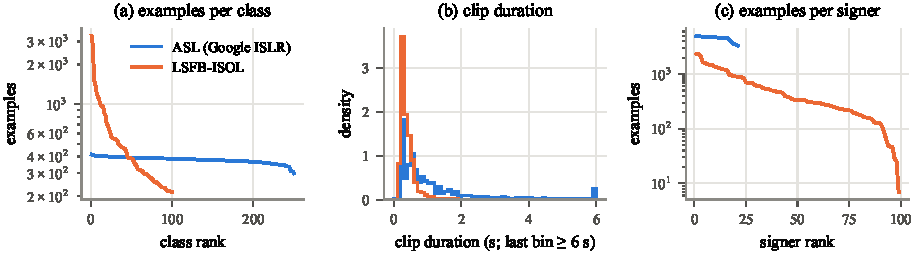
\includegraphics[width=\linewidth]{dataset_overview}
  \caption{Dataset overview. (a) Examples per class, sorted; (b) distribution of clip durations;
  (c) examples per signer, sorted.}
  \label{fig:data-overview}
\end{figure}

\begin{figure}[t]
  \centering
  \begin{minipage}[b]{0.42\linewidth}
    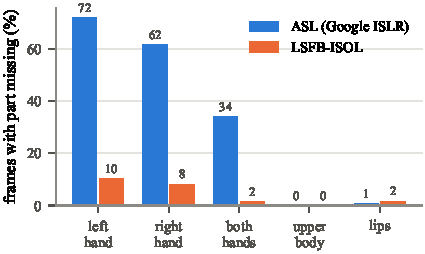
\includegraphics[width=\linewidth]{missing_parts}
    \caption{Share of frames in which a body part is not detected.}
    \label{fig:missing}
  \end{minipage}\hfill
  \begin{minipage}[b]{0.54\linewidth}
    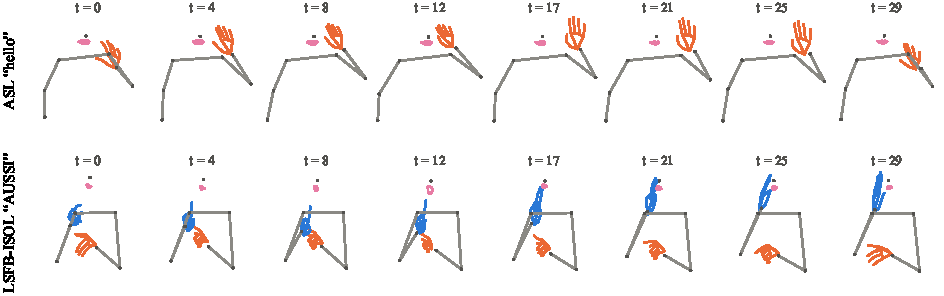
\includegraphics[width=\linewidth]{examples}
    \caption{One ASL and one LSFB clip, eight evenly spaced frames (hand slots in orange and
    blue, lips in pink, upper body in grey).}
    \label{fig:examples}
  \end{minipage}
\end{figure}

\begin{figure}[t]
  \centering
  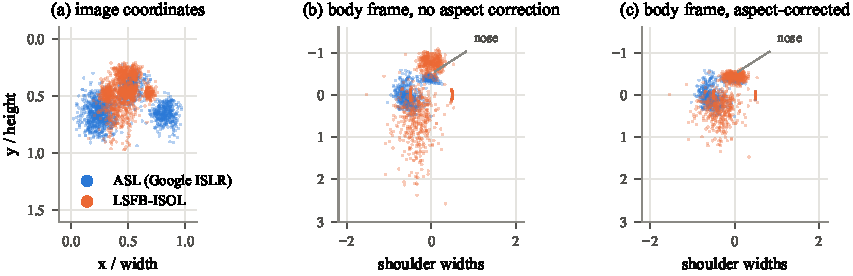
\includegraphics[width=\linewidth]{normalisation}
  \caption{Per-clip mean position of the nose, the shoulders and the dominant wrist for 400 random
  clips of each corpus. (a) Image coordinates; (b) body frame without aspect correction, where the
  LSFB nose lies twice as high as the ASL one; (c) body frame with aspect correction, where both
  corpora align.}
  \label{fig:normalisation}
\end{figure}

\section{Method}
\label{sec:method}

\begin{figure}[t]
  \centering
  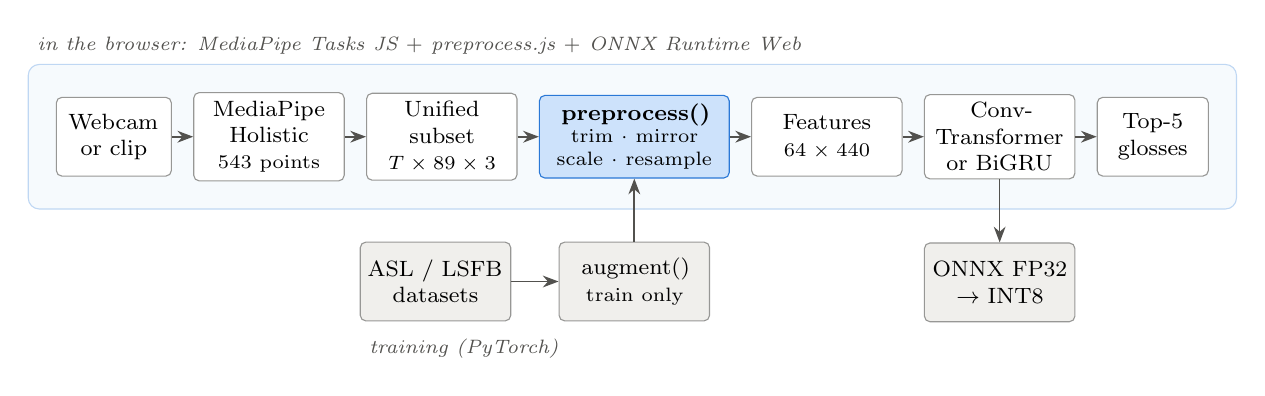
\begin{tikzpicture}[
    font=\footnotesize,
    node distance=4.5mm and 2.7mm,
    box/.style={draw=inkTwo!60, rounded corners=2pt, fill=white, align=center,
                minimum height=10mm, inner sep=3pt, text width=#1},
    box/.default=17mm,
    hl/.style={box=#1, fill=softBlue, draw=sOne},
    hl/.default=17mm,
    arr/.style={-{Stealth[length=2mm]}, draw=inkTwo, line width=0.6pt},
    lab/.style={font=\scriptsize\itshape, text=inkTwo},
  ]
  % main row
  \node[box=12.5mm] (cam) {Webcam\\or clip};
  \node[box, right=of cam] (mp) {MediaPipe\\Holistic\\\scriptsize 543 points};
  \node[box, right=of mp] (sub) {Unified\\subset\\\scriptsize $T\times89\times3$};
  \node[hl=22mm, right=of sub] (pre) {\textbf{preprocess()}\\\scriptsize trim $\cdot$ mirror\\[-1pt]\scriptsize scale $\cdot$ resample};
  \node[box, right=of pre] (feat) {Features\\\scriptsize $64\times440$};
  \node[box, right=of feat] (model) {Conv-Transformer\\or BiGRU};
  \node[box=12mm, right=of model] (out) {Top-5\\glosses};
  \foreach \a/\b in {cam/mp, mp/sub, sub/pre, pre/feat, feat/model, model/out}
    \draw[arr] (\a) -- (\b);

  % training branch
  \node[box=17mm, below=8mm of pre, fill=soft] (aug) {augment()\\\scriptsize train only};
  \node[box=17mm, left=6mm of aug, fill=soft] (data) {ASL / LSFB\\datasets};
  \draw[arr] (data) -- (aug);
  \draw[arr] (aug) -- (pre);
  \node[box=17mm, below=8mm of model, fill=soft] (onnx) {ONNX FP32\\$\to$ INT8};
  \draw[arr] (model) -- (onnx);

  % groupings
  \begin{scope}[on background layer]
    \node[fit=(cam)(mp)(sub)(pre)(feat)(model)(out), inner sep=3.5mm, rounded corners=4pt,
          fill=sOne!4, draw=sOne!30] (rt) {};
  \end{scope}
  \node[lab, anchor=south west] at (rt.north west) {in the browser: MediaPipe Tasks JS $+$ preprocess.js $+$ ONNX Runtime Web};
  \node[lab, anchor=north west] at ($(data.south west)+(0,-1mm)$) {training (PyTorch)};
\end{tikzpicture}

  \caption{System overview. The same preprocessing function serves training (Python) and the
  browser runtime (JavaScript port, tested for parity). Only landmarks are processed; video never
  leaves the device.}
  \label{fig:pipeline}
\end{figure}

\Cref{fig:pipeline} summarises the system. A deterministic preprocessing function maps a raw
landmark sequence to a fixed-size feature matrix, which is augmented during training only and
classified by a sequence model.

\subsection{Preprocessing}
\label{sec:preprocessing}

Let $X\in\mathbb{R}^{T\times L\times3}$ be a raw sequence. Preprocessing applies the following
steps in order.

\paragraph{Temporal trimming.} Leading and trailing frames without any detected hand are removed;
a sequence in which no hand is ever detected is kept unchanged.

\paragraph{Canonical dominant hand.} One-handed signs are produced with the dominant hand, and the
handedness assigned by the landmark estimator depends on whether the image is mirrored. We count
the frames in which each hand slot is detected and, if the left slot is more frequent, mirror the
sequence: $x\mapsto 1-x$ for all points, combined with the permutation $\pi$ that swaps left and
right hands, shoulders, elbows, wrists and symmetric lip points. The resulting features are
invariant to a horizontal flip of the input whenever one hand dominates, a property verified by a
unit test.

\paragraph{Spatial normalisation.} Let $s^{l}_t$ and $s^{r}_t$ denote the shoulder positions in
frame $t$, and $\mathcal{T}_s$ the set of frames in which both are detected. All points are
centred and scaled as
\begin{equation}
  c = \frac{1}{|\mathcal{T}_s|}\sum_{t\in\mathcal{T}_s}\frac{s^{l}_t+s^{r}_t}{2}, \qquad
  w = \frac{1}{|\mathcal{T}_s|}\sum_{t\in\mathcal{T}_s}\lVert s^{l}_t-s^{r}_t\rVert_2, \qquad
  \tilde{X}_{t,j} = \frac{X_{t,j}-c}{w},
\end{equation}
applied to $(x,y)$, with $z$ divided by $w$. Both constants are computed over the whole clip, so
that the motion of the hands relative to the body is preserved. If the shoulders are missing or
degenerate ($w<0.02$), the centroid of all visible points and four times their mean standard
deviation are used instead.

\paragraph{Fixed length.} The clip is linearly resampled to $T'=64$ frames, which also normalises
signing speed and frame rate (30\,fps for ASL, 50\,fps for LSFB). When an interpolation involves a
missing neighbour, the value of the nearest frame is used. Zero-padding with a mask is evaluated as
an alternative in \cref{sec:ablations}.

\paragraph{Features.} Each frame is described by (i) the normalised $(x,y)$ coordinates of the 89
landmarks; (ii) the dominant hand expressed relative to its wrist and divided by the length of the
segment from the wrist to the base of the middle finger, which separates handshape from hand
position; and (iii) the first-order temporal differences of (i) and (ii). Depth is discarded by
default. This yields $F = 2\times(89+21)\times2 = 440$ features per frame. Remaining missing values
are set to zero, i.e.\ missing landmarks are encoded at the body centre.

\subsection{Data augmentation}
Augmentation is applied during training only, in two stages. The first stage acts on the raw
sequence: a time warp combining a global speed change ($\sigma\sim\mathcal{U}[0.8,1.2]$, the clip
being resampled to $T/\sigma$ frames) with a smooth monotonic warp of the time axis over four
segments with relative speeds in $[0.7,1.3]$; random frame dropping ($p=0.1$); random masking of
individual landmarks ($p=0.05$) and of a whole hand in a frame ($p=0.05$); and Gaussian noise
($\sigma=0.002$). The non-uniform component is essential: since every clip is resampled to $T'$
frames, a uniform speed change alone would be almost entirely undone by length normalisation.

The second stage is applied with probability $0.8$ \emph{after} shoulder normalisation, in the
body frame: a rotation of up to $\pm15^\circ$, a per-axis scaling in $[0.8,1.2]$ and a translation
of up to $0.1$ shoulder widths. Applied in image coordinates, before normalisation, translations
and isotropic scalings would be cancelled exactly, as our unit tests confirm. Random draws are
seeded by (seed, epoch, sample) for reproducibility.

\subsection{Models}

\paragraph{Input projection.} Both models first project each frame to $d=192$ dimensions with two
linear layers, layer normalisation and GELU activations.

\paragraph{BiGRU.} Two bidirectional GRU layers \citep{cho2014gru} with 192 hidden units per
direction, followed by masked mean and max pooling over time and a linear classifier
(\numGruParams{}\,M parameters).

\paragraph{Convolution--Transformer.} After a learned positional embedding, the network stacks two
stages, each made of three convolution blocks and one Transformer block
\citep{vaswani2017attention}. A convolution block is a pre-norm residual unit: pointwise expansion
with a gated linear unit \citep{dauphin2017glu}, depthwise temporal convolution with kernel size 17,
batch normalisation, SiLU and pointwise projection, as in the convolution module of the Conformer
\citep{gulati2020conformer}. Transformer blocks use four heads and an MLP ratio of two. The
sequence is mean-pooled under the mask before the classifier (\numTrParams{}\,M parameters).
Attention is implemented with plain matrix products, so that the model exports to ONNX without
custom operators. We refer to this model as the Conv-Transformer.

\subsection{Training}
Models are trained with AdamW \citep{loshchilov2019adamw} (learning rate $10^{-3}$, weight decay
$0.05$, batch size 128), a cosine schedule with three warm-up epochs, label smoothing of $0.1$
\citep{szegedy2016rethinking} and gradient clipping at norm 1, for at most 50 epochs. Early stopping
monitors the validation macro-F1 with a patience of 10 epochs, and the checkpoint with the best
validation macro-F1 is retained. Mixed precision is used on GPU. \Cref{app:hparams} lists all
hyper-parameters.

\paragraph{Transfer.} For cross-lingual transfer, all weights except the classifier are
initialised from the ASL model, and a new classifier is trained for the target vocabulary. Since
the input representation is identical across datasets, no adapter is required. We compare full
fine-tuning with a variant that freezes the encoder during the first five epochs. Two additional
controls test the robustness of the result: fine-tuning with a five times lower learning rate, and
a linear probe in which the encoder stays frozen throughout training.

\subsection{Browser runtime}
\label{sec:runtime}

The demo runs the MediaPipe Holistic Landmarker (Tasks API, WebAssembly with GPU delegate) on the
webcam stream, builds the 89-landmark frame and passes it to a segmenter that detects the start
and end of each sign. The segmenter is a state machine: a sign starts after three consecutive
frames with a visible hand and ends when the hands disappear for six frames, remain still (mean
hand displacement below $0.012$ shoulder widths per frame) for fourteen frames, or after 120
frames. The segment is then preprocessed by the JavaScript port and classified by the ONNX model
with ONNX Runtime Web \citep{onnxruntime} (WebAssembly backend).

Mismatches between training and deployment preprocessing are a common cause of failure in
deployed systems. We therefore generate test fixtures from the Python implementation (missing
hands, mirrored input, missing shoulders, single-frame and long clips, padding, depth features)
and verify that the JavaScript port reproduces the features within \numJsParity{}, i.e.\ at
single-precision accuracy. We also test the complete browser path: executed in headless Chromium
through the code of the demo, the LSFB test clips shipped with the demo receive the same top-1
prediction as with the PyTorch checkpoint (\numBrowserSame{} clips), with probabilities differing
by at most $\numBrowserDiff{}$.

\section{Experimental protocol}
\label{sec:protocol}

\paragraph{Splits.} All splits are \emph{signer-independent} and frozen in version-controlled
files. For ASL, the \numAslSigners{} participants are divided into 14 training, 3 validation and 4
test signers. For LSFB, we keep the official test signers and draw 15\,\% of the official training
signers for validation (\cref{tab:datasets}). To measure leakage (RQ1), we also build a random,
sample-level ASL split with the same proportions, in which every signer appears in all subsets.

\paragraph{Metrics.} We report top-1 and top-5 accuracy, macro-F1 over classes, and the standard
deviation of top-1 accuracy across test signers. Model selection and all ablations rely on the
validation signers; the test signers are used once, to evaluate the final models.

\paragraph{Statistical tests.} Two models evaluated on the same test clips are compared with a
paired bootstrap of their accuracy difference \citep{efron1993bootstrap}, using per-clip
correctness averaged over the three seeds. The \emph{signer-level} bootstrap draws test signers
with replacement and then clips within each drawn signer, so that its 95\,\% interval accounts for
the choice of the test signers; the \emph{clip-level} bootstrap only draws clips within each signer
and treats the signers as fixed. We also apply an exact McNemar test \citep{mcnemar1947note} to the
predictions of the seed ensembles.

\paragraph{Baselines.} Besides chance level, we compute per-coordinate temporal statistics (mean,
standard deviation, minimum and maximum of the normalised position features over the clip,
$4\times220$ features) and classify them with a multinomial logistic regression or with
gradient-boosted trees (LightGBM).

\paragraph{Seeds and compute.} Main models are trained with three seeds and reported as mean
$\pm$ standard deviation; ablations use a single seed. Deep models are trained on one NVIDIA T4 GPU
in a cloud notebook, except for two transfer controls run on the GPU of an Apple M1 laptop once
the cloud quota was exhausted. Latency is measured on the laptop CPU with one thread.

\section{Results}
\label{sec:results}

\subsection{ASL: baselines and sequence models}
\label{sec:results-asl}

\begin{table}[t]
  \centering
  \caption{ASL results (\numAslClasses{} signs). Validation and test sets contain 3 and 4 signers
  absent from training. Sequence models: mean $\pm$ standard deviation over three seeds, 50
  epochs. The last column is the standard deviation of top-1 accuracy across the four test
  signers. All values in \%.}
  \label{tab:main}
  \small
  \begin{tabular}{lcccccc}
\toprule
 & & \multicolumn{1}{c}{Validation} & \multicolumn{4}{c}{Test (4 unseen signers)} \\
\cmidrule(lr){3-3}\cmidrule(lr){4-7}
Model & Params & Top-1 & Top-1 & Top-5 & Macro-F1 & Signer s.d. \\
\midrule
Chance & -- & 0.40 & 0.40 & 2.0 & -- & -- \\
Statistics + log.\ regression & -- & 47.9 & 42.1 & 69.4 & 41.9 & -- \\
Statistics + LightGBM & -- & 45.2 & 33.8 & 61.5 & 33.4 & -- \\
\midrule
BiGRU & 1.43\,M & 65.8 $\pm$ 0.5 & 63.0 $\pm$ 0.5 & 84.0 $\pm$ 0.3 & 62.3 $\pm$ 0.6 & 3.9 $\pm$ 0.4 \\
Conv-Transformer & 2.16\,M & 68.2 $\pm$ 0.1 & 64.8 $\pm$ 0.4 & 84.0 $\pm$ 0.3 & 64.1 $\pm$ 0.4 & 3.3 $\pm$ 0.2 \\
\bottomrule
\end{tabular}

\end{table}

\Cref{tab:main} reports the main comparison. Temporal statistics are already informative: a
logistic regression reaches \numAslLogregTest{}\,\% top-1 on unseen signers, about
\numAslLogregChance{} times chance level. Gradient-boosted trees fit the training signers better
but generalise worse (\numAslLgbmTest{}\,\% on test, \numAslLgbmDrop{} points below their
validation score, against \numAslLogregDrop{} points for the linear model). With only 14
training signers, flexible models on hand-crafted statistics capture signer-specific cues.

Both sequence models exceed the baselines by more than 20 points. The Conv-Transformer reaches
\numTrTestTop{}\,\% top-1 on the test signers and the BiGRU \numGruTestTop{}\,\%, with the same
top-5 accuracy of \numTrTestTopFive{}\,\%. Variation across seeds is small (below one point), whereas variation
across signers is large: accuracy ranges from \numSignerMin{} to \numSignerMax{}\,\% over the four
test signers, and the Conv-Transformer outperforms the BiGRU on each of them
(\cref{fig:signers}a). The difference of \numTrGruDiff{} points is significant even when the test
signers themselves are resampled (signer-level 95\,\% interval
[\numTrGruCiLo{}, \numTrGruCiHi{}]; clip-level [\numTrGruClipCiLo{}, \numTrGruClipCiHi{}];
McNemar \numTrGruMcnemar{}), although four signers remain a small sample. Validation accuracy increases until the end of the 50-epoch schedule
(\cref{fig:curves}), yet a three times longer schedule brings no improvement
(\cref{sec:ablations}): the late gains result from the decay of the learning rate.

\begin{figure}[t]
  \centering
  \begin{minipage}[b]{0.36\linewidth}
    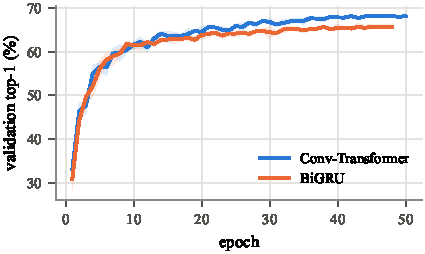
\includegraphics[width=\linewidth]{training_curves}
    \caption{Validation top-1 during training (mean over seeds; band: min--max).}
    \label{fig:curves}
  \end{minipage}\hfill
  \begin{minipage}[b]{0.6\linewidth}
    \centering
    \small
    \captionof{table}{Most frequent confusions of the Conv-Transformer on the ASL test signers
    (seed 0). Rate: share of the clips of the true sign.}
    \label{tab:confusions}
    \begin{tabular}{llrr}
\toprule
True sign & Predicted & Count & Rate \\
\midrule
wake & awake & 40 & 51\,\% \\
pen & pencil & 36 & 45\,\% \\
think & penny & 33 & 43\,\% \\
awake & wake & 31 & 42\,\% \\
duck & goose & 26 & 32\,\% \\
look & see & 24 & 26\,\% \\
say & chin & 23 & 32\,\% \\
scissors & cut & 22 & 33\,\% \\
have & animal & 22 & 31\,\% \\
listen & hear & 21 & 22\,\% \\
lips & mouth & 21 & 28\,\% \\
there & boat & 20 & 27\,\% \\
\bottomrule
\end{tabular}

  \end{minipage}
\end{figure}

\paragraph{Error analysis.}
The most frequent confusions (\cref{tab:confusions}) are linguistically plausible. Several pairs
are near-synonyms that share an identical or very similar sign in many ASL varieties
(\textsc{wake}/\textsc{awake}, \textsc{pen}/\textsc{pencil}, \textsc{look}/\textsc{see}); others
differ by a small change of handshape or location (\textsc{duck}/\textsc{goose},
\textsc{think}/\textsc{penny}). The hardest classes, \numWorstClasses{}, are pointing and
directional signs whose form depends on the location of the referent, which a closed-vocabulary
classifier cannot resolve. Part of the residual error is therefore a property of the vocabulary
rather than of the model.

Landmark quality is the other main factor (\cref{fig:signers}b). Accuracy reaches
\numMissLowAcc{}\,\% when hands are missing in at most 10\,\% of the frames, but falls to
\numMissHighAcc{}\,\% when no hand is detected in more than half of the frames, which concerns
\numMissHighShare{}\,\% of the test clips. Clips with a hand visible in every frame are slightly
less accurate than the next bin because they are shorter (median of \numFullHandFrames{} frames
instead of \numPartHandFrames{}): among them, clips of at most ten frames, which are probably
truncated, are recognised in \numShortAcc{}\,\% of cases, against \numTypicalAcc{}\,\% for clips of
20 to 40 frames.

\begin{figure}[t]
  \centering
  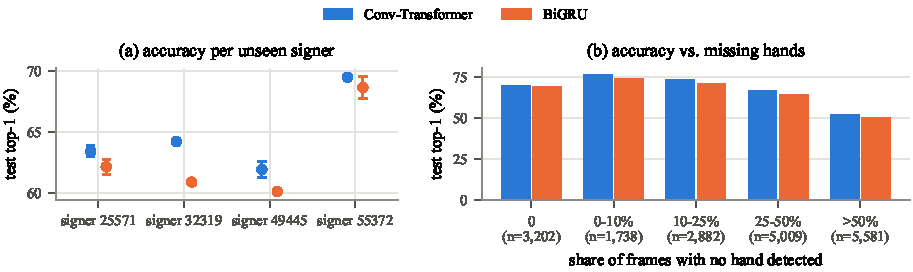
\includegraphics[width=\linewidth]{signers_missing}
  \caption{(a) Test top-1 for each unseen signer (mean and standard deviation over seeds).
  (b) Test top-1 as a function of the share of frames in which neither hand is detected.}
  \label{fig:signers}
\end{figure}

\subsection{Leakage, ablations and training budget}
\label{sec:ablations}

\paragraph{Leakage.}
With a random, sample-level split of the same size, in which every signer appears in both training
and test data, the Conv-Transformer reaches \numLeakRandom{}\,\% test top-1 instead of
\numLeakSigner{}\,\%. A random split thus overestimates the accuracy on new users by \numLeakGap{}
points, more than the effect of any architectural or preprocessing choice studied here.

\paragraph{Ablations.}
\Cref{fig:ablations} changes one factor at a time with respect to the full model
(\numRefValTop{}\,\% validation top-1; seed-to-seed standard deviation of 0.1 point). Early stopping
proved to be a confounding factor. Two variants initially stopped on a validation plateau after 21
and 31 epochs, while the learning rate was still high, and appeared to lose 4.4 and 2.7 points.
Re-run over the full 50-epoch schedule, their effects reduce to \numAblNoHandlocal{} (no hand-local
features) and \numAblXyz{} (depth added) points. The other variants marked with $\dagger$
(\numAblEarlyStopped{} in total) stopped between epochs 41 and 46; their effects may be slightly
overestimated, and our compute budget did not allow re-running them.

Under this caveat, the canonical dominant hand has the largest effect (\numAblNoCanonical{} points
without it): otherwise, the same sign occupies either hand slot depending on the handedness of the
signer and on mirroring. Velocities (\numAblNoVelocity{}), augmentation (\numAblNoAugment{}), depth
(\numAblXyz{}, consistent with the noise of monocular depth estimates) and the hand-local shape
features (\numAblNoHandlocal{}) have moderate effects.

Three findings depart from common practice. First, the lips and the upper body bring no
measurable gain on this vocabulary (\numAblNoLips{} without lips, \numAblHandsOnly{} with hands
only): the 250 signs are mainly distinguished by the hands, and mouthing is presumably rare in
dictionary-like recordings. Second, shorter sequences perform as well ($T'=32$: \numAblTThreeTwo{})
and longer ones no better ($T'=96$: \numAblTNineSix{}), the median clip containing only 22 frames.
Third, zero-padding with a mask outperforms resampling (\numAblPad{}): resampling stretches short
clips and removes the duration cue, whereas padding preserves the original temporal dynamics. The
resampled configuration, fixed before the ablations, is kept in the rest of the study, but padding
is the better choice for future work.

\paragraph{Training budget and ensembles.}
Training the Conv-Transformer for 150 instead of 50 epochs does not help (\numLongVal{}\,\% against
\numRefValTop{}\,\% on validation): the late rise of the curves in \cref{fig:curves} reflects the
annealing of the learning rate, not under-training. Averaging the predictions of the three seeds,
by contrast, improves test top-1 to \numAslEnsTop{}\,\% on ASL (\numTrTestTopMean{}\,\% for a
single model) and to \numLsfbEnsTop{}\,\% on LSFB (\numLsfbScratchTest{}\,\%), at three times the
inference cost.

\begin{figure}[t]
  \centering
  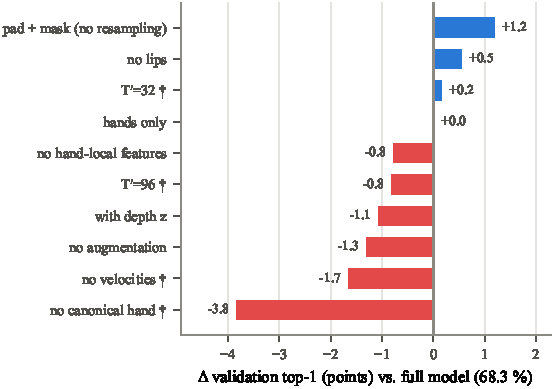
\includegraphics[width=0.62\linewidth]{ablations}
  \caption{One-factor ablations of the Conv-Transformer on the ASL validation signers (seed 0).
  $\dagger$: early stopping ended the run before the end of the 50-epoch schedule (epochs 41--46),
  so the effect may be overestimated.}
  \label{fig:ablations}
\end{figure}


\subsection{Cross-lingual transfer to LSFB}
\label{sec:transfer}

\Cref{tab:transfer} reports the results on LSFB-ISOL with all training data. Trained from scratch,
the Conv-Transformer reaches \numLsfbScratchTest{}\,\% top-1 and \numLsfbScratchTestFOne{}\,\%
macro-F1 on the 40 official test signers, well above the statistical baselines (\numLsfbLogregTest{}\,\% and
\numLsfbLogregTestFOne{}\,\%). Macro-F1 is markedly lower than top-1 on this corpus because of its long tail: the ten
most frequent glosses account for \numLsfbTopTenShare{}\,\% of the test clips.

\paragraph{Validation and test accuracy.}
On LSFB, validation accuracy exceeds test accuracy by far more than on ASL (\numGapValClip{} against
\numGapTestClip{}\,\%). The validation set is small and unbalanced across signers: three of its
\numGapValSigners{} signers contribute \numGapTopThreeShare{}\,\% of its clips. Averaged per signer,
accuracy is \numGapValPerSigner{}\,$\pm$\,\numGapValPerSignerSem{}\,\% on validation (seed 0) and
\numGapTestPerSigner{}\,$\pm$\,\numGapTestPerSignerSem{}\,\% on test (mean over seeds; mean $\pm$
standard error over signers), and re-weighting the test clips to the class distribution of the validation set raises
test accuracy to \numGapTestReweighted{}\,\%. LSFB clips come from dialogues: test signers whose
conversation partner belongs to the training signers (\numGapTestPartnerInN{} of
\numGapTestSigners{}) are recognised with \numGapTestPartnerIn{}\,\% accuracy, the others with
\numGapTestPartnerOut{}\,\%, which suggests that shared conversations, and therefore shared topics
and signing styles, also favour held-out signers. Validation scores are therefore used only to
compare configurations, never as an estimate of performance on new signers.

\paragraph{ASL pre-training.}
Initialising the encoder from the ASL model does not improve recognition. With all training data,
fine-tuning the ASL model yields \numLsfbFtTest{}\,\% (\numLsfbFtVal{}\,\% on validation, against
\numLsfbScratchVal{}\,\% from scratch), and freezing the encoder during the first five epochs only
narrows the gap (\numLsfbFreezeTest{}\,\%). Pre-training is not merely useless but slightly harmful: relative to training from scratch,
test accuracy changes by \numLsfbFtDiff{} points with fine-tuning (signer-level 95\,\% interval
[\numLsfbFtCiLo{}, \numLsfbFtCiHi{}], \numLsfbFtP{}) and by \numLsfbFreezeDiff{} points with the
frozen variant ([\numLsfbFreezeCiLo{}, \numLsfbFreezeCiHi{}]). The learning curves of \cref{fig:transfer} show that
this result does not depend on the size of the training set. Both initialisations are
indistinguishable from 5 to 25 examples per sign (the largest difference, \numGainFew{} points at
5 examples, lies within one seed standard deviation), and the model trained from scratch leads
from 50 examples per sign onwards, by \numScratchLeadAll{} points with all data.

\paragraph{Controls.}
Two controls exclude an inadequate fine-tuning procedure as the explanation. First, a linear probe
trained on top of the frozen ASL encoder with all LSFB training data reaches \numProbeAll{}\,\%
validation top-1, far below the model trained from scratch (\numLsfbScratchVal{}\,\%) and even
below the logistic regression on temporal statistics (\numLsfbLogregVal{}\,\%). The ASL
representation therefore retains some information about LSFB signs, but less than simple features
of the target data. Second, with 25 examples per sign, fine-tuning with a five times lower
learning rate gives \numLowlrTwentyFive{}\,\% validation top-1, below both standard fine-tuning
(\numFtTwentyFive{}\,\%) and training from scratch (\numScratchTwentyFive{}\,\%) with the same seed.
Both controls use a single seed, and every transfer run starts from the ASL model of seed 0, so
the variability of the pre-trained model itself is not sampled. During the linear probe, the
batch-normalisation statistics of the frozen encoder were still updated on LSFB, a mild form of
adaptation; the probe is therefore, if anything, favoured, which does not change its conclusion.

\begin{figure}[t]
  \centering
  \begin{minipage}[b]{0.44\linewidth}
    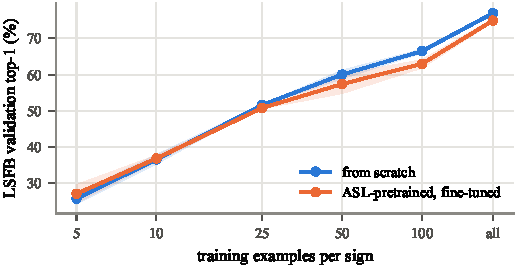
\includegraphics[width=\linewidth]{transfer_curve}
    \caption{LSFB validation top-1 as a function of the number of training examples per sign
    (mean $\pm$ s.d.\ over three seeds). ``All'' corresponds to a median of \numLsfbMedianPerClass{} examples per
    sign.}
    \label{fig:transfer}
  \end{minipage}\hfill
  \begin{minipage}[b]{0.53\linewidth}
    \centering
    \small
    \captionof{table}{LSFB-ISOL, 100 glosses, all training data. Mean $\pm$ s.d.\ over three
    seeds, values in \%.}
    \label{tab:transfer}
    \resizebox{\linewidth}{!}{\begin{tabular}{lcccc}
\toprule
 & Validation & \multicolumn{3}{c}{Test (40 unseen signers)} \\
\cmidrule(lr){2-2}\cmidrule(lr){3-5}
Model & Top-1 & Top-1 & Top-5 & Macro-F1 \\
\midrule
Chance & 1.0 & 1.0 & 5.0 & -- \\
Statistics + log.\ regression & 57.0 & 49.0 & 75.3 & 40.9 \\
Statistics + LightGBM & 54.8 & 47.1 & 72.6 & 37.3 \\
\midrule
Conv-Transformer, from scratch & 77.0 $\pm$ 0.3 & 68.3 $\pm$ 0.2 & 87.7 $\pm$ 0.1 & 63.9 $\pm$ 0.2 \\
\quad ASL-pretrained, fine-tuned & 74.9 $\pm$ 0.4 & 66.2 $\pm$ 0.2 & 87.1 $\pm$ 0.4 & 61.7 $\pm$ 0.3 \\
\quad ASL-pretrained, encoder frozen 5 epochs & 75.6 $\pm$ 0.6 & 66.6 $\pm$ 0.2 & 86.5 $\pm$ 0.5 & 62.0 $\pm$ 0.3 \\
\bottomrule
\end{tabular}
}
  \end{minipage}
\end{figure}


\subsection{Efficiency and deployment}
\label{sec:efficiency}

\begin{table}[t]
  \centering
  \caption{Model size and single-sign latency on an Apple M1 CPU (one thread) after export to
  ONNX. Native: ONNX Runtime; browser: ONNX Runtime Web (WebAssembly) in Chromium. INT8: dynamic
  quantisation of the weight matrices, with the input projection kept in FP32. Validation top-1
  on 2{,}000 ASL validation clips.}
  \label{tab:export}
  \small
  \begin{tabular}{llrrrrr}
\toprule
 & & & Native & \multicolumn{2}{c}{Browser (WebAssembly)} & \\
\cmidrule(lr){5-6}
Model & Precision & Size & p50 (ms) & p50 (ms) & p95 (ms) & Val.\ top-1 \\
\midrule
Conv-Transformer & FP32 & 8.3\,MB & 7.8 & 16.3 & 22.0 & 67.8 \\
Conv-Transformer & INT8 & 2.5\,MB & 16.5 & 33.4 & 44.8 & 68.3 \\
BiGRU & FP32 & 5.5\,MB & 5.7 & 7.9 & 11.0 & -- \\
BiGRU & INT8 & 4.8\,MB & 5.5 & 8.1 & 10.2 & -- \\
\bottomrule
\end{tabular}

\end{table}

\paragraph{Latency.}
\Cref{tab:export} summarises the inference cost. Preprocessing takes about 0.3\,ms per clip in
Python, and each sign is classified once, when the segmenter detects its end. The
Conv-Transformer then requires \numFpNative{}\,ms natively and \numFpBrowser{}\,ms in the browser,
and the BiGRU \numGruBrowser{}\,ms in the browser. Landmark extraction by MediaPipe, which runs on
every frame, dominates the cost of the live demo.

\paragraph{Quantisation.}
Naive dynamic INT8 quantisation reduces the validation top-1 of the Conv-Transformer from 68\,\% to
34\,\%. The cause is a small number of very large inputs: when a detected hand is tiny, the
hand-local features (\cref{sec:preprocessing}) are divided by a near-zero length and reach values
close to 200, while 99.9\,\% of them remain below 6.2. A per-tensor dynamic scale on the first
layer then destroys the resolution of all other inputs. Keeping this single layer in FP32 fully
restores accuracy. The quantised model is \numIntShrink{}$\times$ smaller but
\numIntSlowdown{}$\times$ \emph{slower} on CPU, natively and in WebAssembly: at this scale,
quantising and dequantising activations around many small matrix products costs more than integer
arithmetic saves. Since the demo already downloads about 25\,MB for MediaPipe, it ships the FP32
model.

\begin{figure}[t]
  \centering
  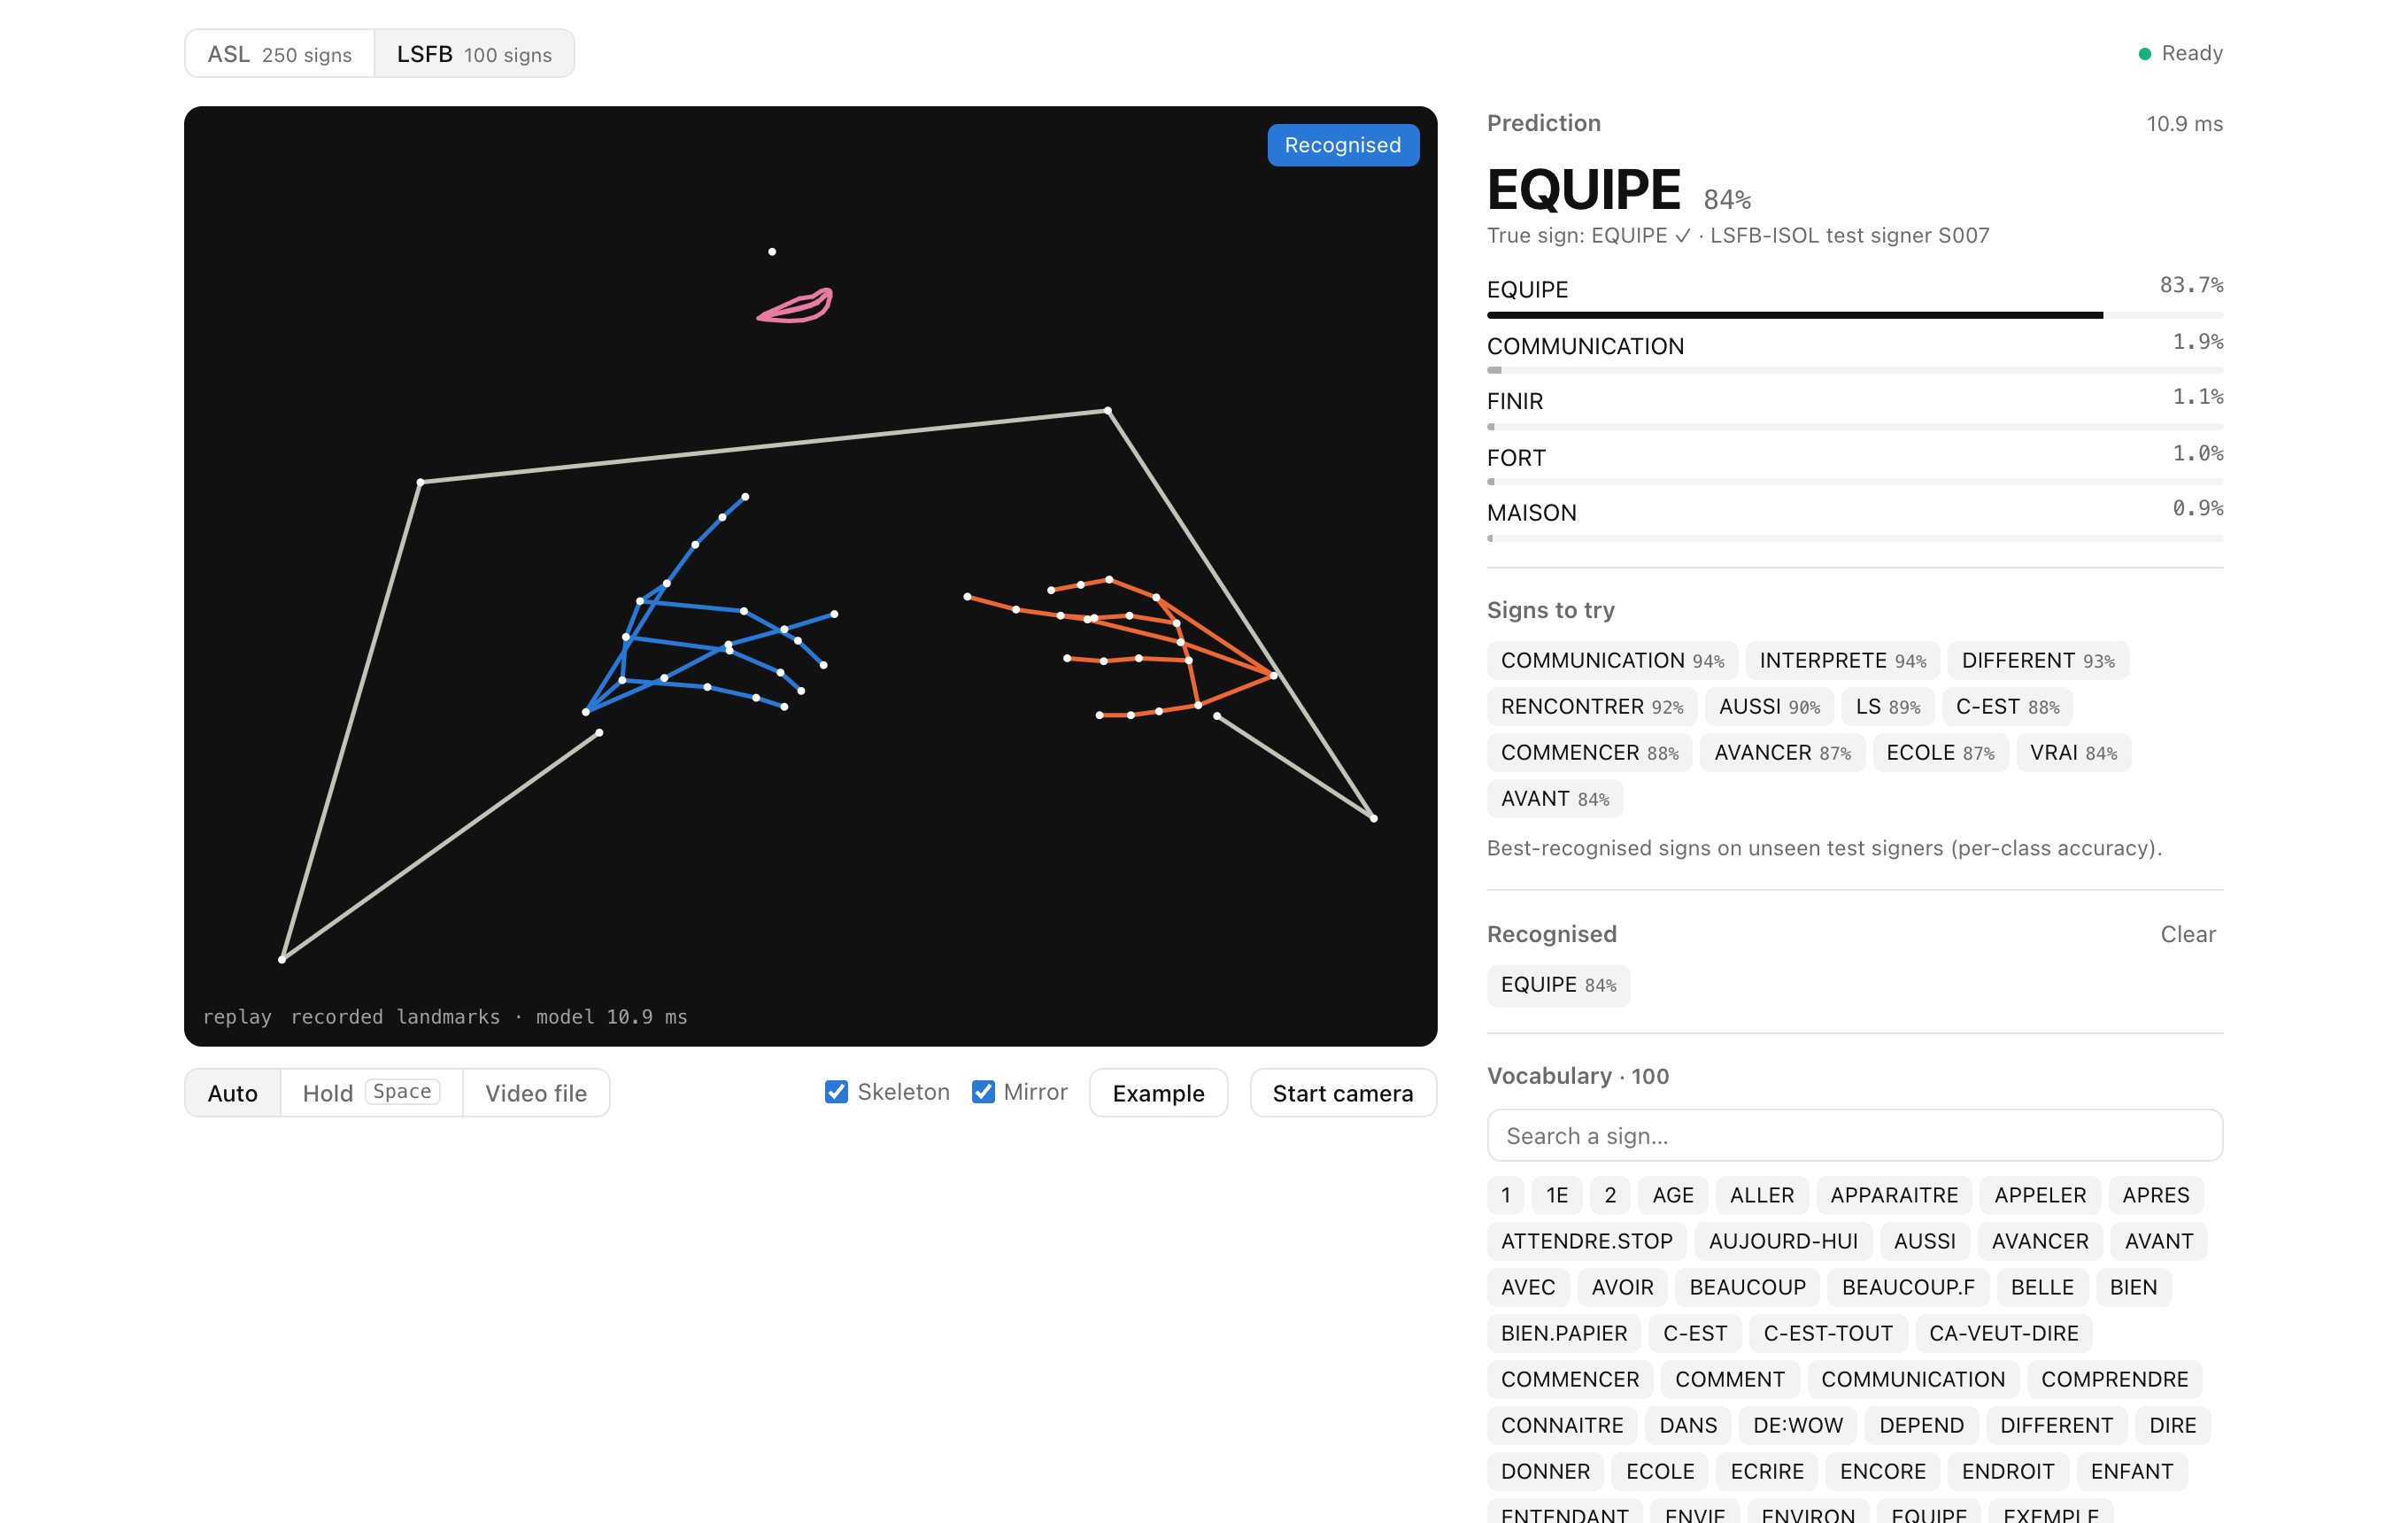
\includegraphics[width=\linewidth]{demo}
  \caption{Browser demo replaying an LSFB-ISOL clip of an unseen test signer: skeleton, top-5
  predictions with the true sign, best-recognised signs, history and vocabulary. The demo ships
  one test clip for each of 40 glosses, of which the model recognises \numExampleAcc{}\,\%. With a
  webcam, signs are segmented automatically from hand presence and motion.}
  \label{fig:demo}
\end{figure}

\section{Discussion}
\label{sec:discussion}

\paragraph{Sources of error.}
All results are obtained on people absent from training, a setting that \cref{sec:ablations} shows
to be considerably harder than a random split suggests. The remaining errors have three main
sources, which call for different remedies: signs that are genuinely ambiguous within a closed
vocabulary (near-synonyms, pointing and directional signs); landmark detection failures, which
dominate the hardest clips; and variation between signers, which exceeds the difference between
the two architectures. More signers and better hand tracking are therefore likely to help more
than a larger classifier.

\paragraph{Absence of transfer from ASL.}
We expected an ASL encoder to help, at least with few LSFB examples, since both languages build
signs from handshapes, movements and locations. The two corpora, however, differ in more than the
language. ASL clips are citation forms recorded one at a time on a smartphone; LSFB clips are
extracted from spontaneous conversations filmed in a studio, are less than half as long (median
\numLsfbDurMedian{}\,s against \numAslDurMedian{}\,s) and are co-articulated with neighbouring signs.
Hands are missing in \numAslNoHandPct{}\,\% of the ASL frames but in \numLsfbNoHandPct{}\,\% of the LSFB
frames, and the landmarks come from two
generations of MediaPipe. The pre-trained encoder is therefore adapted to a different input
distribution, and even a few hundred labelled clips of the target corpus provide more relevant
information than this prior. This explanation is consistent with our measurements but not
demonstrated: separating the effect of the language from that of the recording conditions would
require a second ASL corpus of conversational signs, or an LSFB corpus of citation forms.
Self-supervised pre-training on unlabelled, in-domain continuous signing, for instance LSFB-CONT
\citep{fink2021lsfb} or MEDIAPI-SKEL \citep{bull2020mediapi} for French Sign Language, appears to be
a more promising direction than supervised cross-lingual pre-training.

\paragraph{Methodological pitfalls.}
Several of our observations are inexpensive to check yet easily overlooked. (i) Image-space
translation and scaling augmentations are cancelled by body-centred normalisation and must be
applied after it. (ii) Normalised landmark coordinates are anisotropic whenever pixels or frames
are not square, which distorts the body frame across datasets. (iii) Early stopping on a plateau
while the learning rate is still high can make an ablation appear much more harmful than it is.
(iv) Rare feature outliers, harmless in floating point, can break post-training quantisation, and
quantisation does not necessarily make a small model faster on CPU. (v) A preprocessing function
implemented in two languages must be tested for parity, which costs little once fixtures are
generated from the reference implementation.

\paragraph{Limitations.}
(i) The ASL test set contains only four signers, so per-signer estimates are uncertain, and all
LSFB clips come from a single corpus recorded in one studio setting. (ii) Both vocabularies are
small and fixed: an out-of-vocabulary sign is always mapped to the closest known sign, and the demo
has no rejection class. (iii) Our ASL accuracy remains well below that of the best competition
solutions \citep{kaggle_islr}, which relied on stronger regularisation and augmentation, much
longer schedules and ensembles of several models, and were trained on all 21 participants, whereas
our models see 14 of them and are tested on a different set. We did not measure how much each of
these factors contributes. A longer schedule alone did not help our model, and the ablations used a
single seed, \numAblEarlyStopped{} of them ending before the full schedule; differences of about one
point between ablations should therefore not be over-interpreted. (iv) Because every clip is
stretched to 64 frames, velocities are expressed per resampled frame: their scale depends on the
duration of the clip and on the frame rate of the source (30 or 50\,fps), which may partly explain
why padding performed better in the ablations. Resampling to a common frame rate and padding would
remove this dependence. (v) The lip contour is the only non-manual information used; eyebrows, gaze and head
movements, which carry grammatical information, are ignored. (vi) The demo segments signs from hand
presence and motion, which suits signs produced one at a time with a pause but not natural,
continuous signing. (vii) No Deaf signer took part in the evaluation of the demo; its usefulness
for the community remains to be established with its members.

\paragraph{Ethical considerations.}
Both datasets were released for research by their creators, under the Kaggle competition rules and
the CC BY 4.0 licence (LSFB-ISOL). ASL data are never redistributed; the demo ships a few LSFB clips
with attribution. The demo processes video locally and stores nothing. Face and body landmarks can
nonetheless identify a person, so any extension that records them should obtain explicit consent.
We describe the system as \emph{isolated sign recognition}: presenting such a classifier as a
translator would mislead users about its capabilities and could cause harm where communication
matters. A model card summarising intended uses, out-of-scope uses and known biases accompanies
the code \citep{mitchell2019modelcards}.

\section{Conclusion}
\label{sec:conclusion}

We built and evaluated an isolated sign recognition system based on MediaPipe landmarks, under a
signer-independent protocol and with a fully client-side deployment. The three research questions
receive the following answers.

\paragraph{RQ1 Generalisation.} A 2.2\,M-parameter convolution--Transformer recognises
\numAslClasses{} ASL signs produced by unseen signers with \numTrTestTop{}\,\% top-1 accuracy, and
\numLsfbClasses{} LSFB glosses with \numLsfbScratchTest{}\,\%. A random split inflates the ASL
accuracy by \numLeakGap{} points, and an early-stopping artefact had overstated the effect of one
ablation fivefold: evaluation choices influence conclusions more than most design choices.

\paragraph{RQ2 Transfer.} Pre-training on ASL does not improve LSFB recognition at any
training-set size, even with five examples per sign, and with all training data it lowers test
accuracy by a small but significant margin. Differences in recording and elicitation
conditions likely outweigh what the two languages share at the level of pose features.

\paragraph{RQ3 Deployment.} The complete pipeline runs in a web browser, classifies a sign in
\numFpBrowser{}\,ms on one CPU thread and reproduces the predictions of the PyTorch model on every
tested clip. INT8 quantisation reduces model size but not latency on CPU.

Future work includes self-supervised pre-training on in-domain continuous signing, a rejection
class for out-of-vocabulary signs, richer non-manual features, and an evaluation of the demo with
Deaf signers.


\bibliographystyle{abbrvnat}
\bibliography{references}

\appendix
\section{Hyper-parameters}
\label{app:hparams}

\begin{table}[!ht]
  \centering
  \caption{Hyper-parameters shared by all experiments unless stated otherwise. All values are
  read from the configuration files released with the code.}
  \label{tab:hparams}
  \small
  \begin{tabular}{llp{5.0cm}}
    \toprule
    Group & Parameter & Value \\
    \midrule
    Preprocessing & frames $T'$ / length mode & 64 / linear resampling \\
                  & coordinates & $(x, y)$; depth dropped \\
                  & landmark parts & both hands, upper body (7 points), lips (40 points) \\
                  & features per frame & positions, dominant-hand local shape, velocities ($F=440$) \\
    \midrule
    Augmentation  & spatial (body frame), probability & 0.8 \\
                  & rotation / per-axis scale / shift & $\pm15^\circ$ / $[0.8, 1.2]$ / $\pm0.1$ shoulder widths \\
                  & global speed / local warp & $[0.8, 1.2]$ / $\pm30\,\%$ over 4 segments \\
                  & frame / landmark / hand dropping & 0.1 / 0.05 / 0.05 \\
                  & Gaussian noise (image units) & 0.002 \\
    \midrule
    BiGRU         & input projection / hidden / layers & 192 / 192 per direction / 2 \\
                  & pooling / dropout & masked mean $\Vert$ max / 0.3 \\
    \midrule
    Conv-Transformer & width / stages & 192 / 2 \\
                  & per stage & 3 conv.\ blocks + 1 Transformer block \\
                  & kernel / expansion / heads / MLP ratio & 17 / 2 / 4 / 2 \\
                  & dropout & 0.2 \\
    \midrule
    Optimisation  & optimiser & AdamW, lr $10^{-3}$, weight decay 0.05 \\
                  & schedule & 3 warm-up epochs, cosine decay \\
                  & batch / max.\ epochs / patience & 128 / 50 / 10 (validation macro-F1) \\
                  & label smoothing / gradient clipping & 0.1 / 1.0 \\
                  & precision & mixed (fp16) on GPU \\
    \bottomrule
  \end{tabular}
\end{table}

\section{Landmark subset}
\label{app:landmarks}

\begin{table}[!ht]
  \centering
  \caption{Unified landmark subset, in the order used by the model (MediaPipe indices).}
  \small
  \begin{tabular}{lrl}
    \toprule
    Part & Points & MediaPipe indices \\
    \midrule
    Left hand & 21 & hand model 0--20 \\
    Right hand & 21 & hand model 0--20 \\
    Upper body & 7 & pose 0 (nose), 11--12 (shoulders), 13--14 (elbows), 15--16 (wrists) \\
    Lips & 40 & face mesh: outer contour (20) and inner contour (20) \\
    \midrule
    Total & 89 & \\
    \bottomrule
  \end{tabular}
\end{table}


\end{document}
